\section{Betrachtung der Komponenten}
\subsection{Mikrocontroller}
Die zentrale Komponente der Digitaluhr ist der Mikrocontroller ATmega32. Der von Atmel hergestellte 8-bit Kontroller ist im 40-pin DIP Format verfügbar. Dies ermöglicht die einfache Verwendung auf einer Lochrasterplatine mit 2,54mm Lochabstand. Programmiert wird der ATMega entweder in C oder in AVR-Assembler, die Wahl fiel hier auf die konfortablere Sprache C.
Viele der integrierten Komponenten wurden genutzt: Das zur Verfügung gestellte SPI-Interface \footnote{Serial Peripheral Interface Bus}zur Kommunitkation mit den Schieberegistern, der integrierte AD-Wandler zur Auswertung des Helligkeitssensors, das ISP-Interface zur Programmierung. TODO: Gibts hier noch mehr?
\begin{table}[htp]
  \renewcommand{\arraystretch}{1.2}
  \begin{tabular}{||l | l||}
  \hline\hline
  Bezeichnung&ATMEGA32 16PU 0926D\\\hline
  Hersteller&Atmel\\\hline
  Architektur&AVR 8-bit \\\hline
  Geschwindigkeit&bis 16Mhz \\\hline
  Programmspeicher&32 KiB Flash \\\hline
  Arbeitsspeicher&2 KiB SRAM \\\hline
  EEPROM&1 KiB \\\hline
  AD-Wandler&8 Kanal / 10 Bit \\\hline
  Bauform&40-pin DIP Gehäuse \\
  \hline\hline    
\end{tabular}
\caption{Eckdaten des ATmega 32}
\end{table}

\subsection{DCF77 Empfangsmodul}\label{sec_dcf77modul}
TODO

\subsection{LED Matrix}
TODO
LEDs: Weiter winkel um gute ausleuchtung zu erhalen

\subsection{Helligkeitssensor}
Ein Fotoresitor (Lichtabhaengier Widerstand) bildet einen Teil eines Spannugteilers. Die innerhalb des Spanungsteilers anliegende Spannung wird dann vom Mikrocontroller mit Hilfe des AD-Wandlers ausgewertet.
Der verwendete Fotoresisor besitzt nominal einen Dunkelwiderstand von $100 k\Omega$ .
Um den Widerstandsverlauf besser abschätzen zu können wurden Messungen vorgenommen.
\begin{table}[htp]
\begin{tabular}{||l | l||}
  \hline \hline
  Dunkelheit& $70 k\Omega$ \\ \hline
  Zimmerhelligkeit & $3 k\Omega$ \\ \hline
  Schreibtischlampe 50cm Abstand& $500 \Omega$ \\ \hline
  Schreibtischlampe 10cm Abstand& $90 \Omega$ \\ \hline
  Schreibtischlampe 2cm Abstand& $30 \Omega$  \\
  \hline\hline
\end{tabular}
\caption{Widerstandmessung des LDR}
\end{table}
  
\subsection{Temperatursensor}
Als Temperatursensor wurde der DS18S20\footnote{\url{http://www.maximintegrated.com/datasheet/index.mvp/id/2815}} von Maxim Integrated verwendet. Dieser verwendet das 1-Wire\textsuperscript{\textregistered}-Protokoll\footnote{\url{http://www.maximintegrated.com/products/1-wire/flash/overview/index.cfm}}, sodass nur ein Datenpin vonnöten ist, worüber Befehle gesendet sowie Daten empfangen werden.

\begin{figure}[htp]
\centering
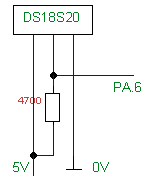
\includegraphics{skizzen/temperatursensor_schematic.png}
\caption{Schaltung für den 1-Wire Temperatursensor}\label{fig_tempsensor}
\end{figure}

\subsection{Infrarotsensor}
%TODO to be removed
\begin{table}[htp]
\centering
\renewcommand{\arraystretch}{1.2}
\begin{tabular}{||l|l||}
\hline \hline
Bezeichnung&ATMEGA32 16PU 0926D\\ \hline
Hersteller&Atmel\\ \hline
Architektur&AVR 8-bit\\ \hline
Geschwindigkeit&bis 16Mhz \\ \hline
Programmspeicher&32 KiB Flash \\ \hline
Arbeitsspeicher&2 KiB SRAM \\ \hline
EEPROM&1 KiB \\ \hline
AD-Wandler&8 Kanal / 10 Bit \\ \hline
Bauform&40-pin DIP Gehäuse\\
\hline\hline
\end{tabular}
\caption{Eckdaten des ATmega 32}
\end{table}

\subsection{Gehäuse}
%TODO
%
Ziel war es ein optisch ansprechendes, sowie funktionales Gehäuse zu kreieren. 

Als problematisch stellte sich die Zielsetzung der flachen Bauart hrraus. Denn um eine gleichmässige Lichtverteilung innerhalb eines Pixels zu erreichen, muss ein relativ großer Abstand zur LED gegeben sein. Durch praktisches Testen ergab sich für die verwendeten LEDs ein idealer Abstand von .%TODO eventuell wirklich probieren 
Auserdem muss verhindert werden, dass die offenliegende Verdrahtung der LED-Matrix zu Kurzschlüssen führt. Im Besonderen ist hier das Netzteil zu nennen, da hier ein Spannung von 230 Volt anliegt und das Netzteil von allen Komponenten mit 15 mm %TODO 
über die höchste Bauhöhe verfügt. 
Die Bauhöhe der Verdrahtung der LED-Matrix wurde an den kritischen Stellen von 5-6 mm auf ca. 2 mm verringert. Um Kurzschlüsse innerhalb der LED-Matrix zu verhindern, wurden die Kreuzungspunkte zum Teil isoliert.
%TODO [MH] evtl Bild davon?

Während der Entwicklung war ein einfacher Zugang von großer Bedeutung, deshalb wurde das Gehäuse in zwei Teile aufgeteilt. Die LED-Matrix bildet zusammen mit ihrer Abdeckung und drei Seitenwänden den vorderen Teil des Gehäuses. Auf der Rückwand wurde die Hauptplatine, das Netzteil und der DCF77-Empfänger platziert. An der vierten Seitenwand sind die Sensoren für Helligkeit und Temperatur, die Stromversorgung, die 6 Taster sowie der Debuganschluss (ISP) %TODO ISP als Fachwort
befestigt. Diese Seitenwand wurde an der Rückwand befestigt. Dies ermöglicht ein Öffnen des Gehäuses, indem nur die Schrauben an der Rückwand entfernt werden und die 3 Steckverbinder zur LED-Matrix gelöst werden, die komplette Sensorik und die Taster aber nicht entfernt werden müssen.
%TODO Fotos von dem ganzen Kram

Als Schrauben kamen Metallschrauben mit M5 %TODO 
Gewinde zum Einsatz. Die Muttern wurden in einem Holzblock befestigt, der anschließend mit der Rückwand verleimt wurde.%TODO: Abbildung? 
Diese Lösung zeichnet sich im Gegensatz zu Holzschrauben durch minimalen Verschleis aus und kann oft geöffnet und wieder verschlossen werden ohne Auszufransen.

\subsubsection{Energieversorgung und Verbrauch}
%TODO: Tabelle mit Alle AN/ Alle Aus/ Halb an. (eventuell mit neuen und alten Widerständen 
Als Netzteil wurde ein CE geprüftes 5V/2A Netzteil gewählt. Das kompakte verwendete Schaltnetzteil ist ausreichend dimensioniert um den, mit einem Labornetzteil, ermittelten maximalen Bedarf von ca. 1.8A%TODO
(alle LEDs an bei maximaler Helligkeit) bereitzustellen.
 
Als Stromkabel kommt ein zweipoliges Kabel mit Schalter zum Einsatz. Dieses wurde im Inneren des Gehäuses mit Schmelzklebestoff verklebt und in eine Lüsterklemme geführt, so dass bei eventuell auftretenden Zugkräften auf keinen Fall Kräfte auf das Netzteil wirken.

Mittels des Temperatursensors wurde außerdem in einem Testlauf sichergestellt, dass die Temperatur im Inneren der Uhr 50\degree C (bei einer Raumtemperatur von 22\degree C) nicht überschreitet.
%eof